
\chapter{Planetary Systems}

\lettrine[lines=4]{\goudy T}{he} solar system, that is to say, the variously formed matter circling round the Sun, consists, according to the present state of our knowledge, of eleven primary planets,\footnote{[Since the publication of Baron Humboldt's work in 1845, several other planets have been discovered, making the number of those belonging to our planetary system sixteen instead of eleven. Of these, Astrea, Hebe, Flora, and Iris are members of the remarkable group of asteroids between Mars and Jupiter. Astrea and Hebe were discovered by Hencke at Driesen, the one in 1846 and the other in 1847; Flora and Iris were both discovered in 1847 by Mr. Hind, at the South Villa Observatory, Regents Park. It would appear from the latest determinations of their elements, that the small planets have the following order with respect to mean distance from the Sun: Flora, Iris, Vesta, Hebe, Astrea, Juno, Ceres, Pallas. Of these, Flora has the shortest teens (about 34 years). The planet Neptune, which, after having been predicted by several astronomers, was actually observed on the 25th of September, 1846, is situated on the confines of our planetary system beyond Uranus. The discovery of this planet is not only highly interesting from the importance attached to it as a question of science, but also from the evidence it affords of the care and unremitting labor evinced by modern astronomers in the investigation and comparison of the older calculations, and the ingenious application of the results thus obtained to the observation of new facts. The merit of having paved the way for the discovery of the planet Neptune is due to M. Bouvard, who, in his persevering and assiduous efforts to deduce the entire orbit of Uranus from observations made during the forty years that succeeded the discovery of that planet in 1781, found the results yielded by theory to be at variance with fact, in a degree that had no parallel in the history of astronomy. This startling discrepancy, which seemed only to gain additional weight from every attempt made by M. Bouvard to correct his calculations, led Leverrier, after a careful modification of the tables of Bouvard, to establish the proposition that there was a formal incompatibility between the observed motions of Uranus and the hypothesis that he was acted on only by the Sun and known planets, according to the law of universal gravitation. Pursuing this idea, Leverrier arrived at the conclusion that the disturbing cause must be a planet, and, finally, after an amount of labor that seems perfectly overwhelming, he, on the 31st of August, 1846, laid before the French Institute a paper, in which he indicated the exact spot in the heavens where this new planetary body would be found, giving the following data for its various elements mean distance from the Sun, 36154 times that of the Earth; period of revolution, 217387 years; mean long., Jan. Ist, 1847, 3189 47; mass, gy55th; heliocentric long., Jan. Ist, 1847, 326 32. Essential difficulties still intervened, however, and as the remoteness of the planet rendered it improbable that its disk would be discernible by any telescopic instrument, no other means remained for detecting the suspected body but its planetary motion, which could only be ascertained by mapping, after every observation, the quarter of the heavens scanned, and by a comparison of the various maps. Fortunately for the verification of Leverrier's predictions, Dr. Bremiker had just completed a map of the precise region in which it was expected the new planet would appear, this being one of a series of maps made for the Academy of Berlin, of the small stars along the entire zodiac. By means of this valuable assistance, Dr. Galle, of the Berlin Observatory, was led, on the 25th of September, 1846, by the discovery of a star of the eighth magnitude, not recorded in Dr. Bremiker's map, to make the first observation of the planet predicted by Leverrier. By a singular coincidence, Mr. Adams, of Cambridge, had predicted the appearance of the planet simultaneously with M. Leverrier; but by the concurrence of several circumstances much to be regretted, the world at large were not made acquainted with Mr. Adams's valuable discovery until subsequently to the period at which Leverrier published his observations. As the data of Leverrier and Adams stand at present, there is a discrepancy between the predicted and the true distance, and in some other elements of the planet; it remains, therefore, for these or future astronomers to reconcile theory with fact, or perhaps, as in the case of Uranus, to make the new planet the means of leading to yet greater discoveries. It would appear from the most recent observations, that the mass of Neptune, instead of being, as at first stated, 5,',,th, is only about sg) yah that of the Sun, while its periodic time is now given with a greater probability at 166 years, and its mean distance from the Sun nearly 30. The planet appears to have a ring, but as yet no accurate observations have been made regarding its system of satellites. See Trans. Astrau. Soc., and The Planet Neptune, 1848, by J. P. Nicholl.]} eighteen satellites or secondary planets, and myriads of comets, three ofwhich, known as the  planetary comets, do not pass beyondthe narrow limits of the orbits described by the principalplanets. We may, with no inconsiderable degree of probability, include within the domain of our Sun, in the immediate sphere of its central force, a rotating ring of vaporous matter, lying probably between the orbits of Venus and Mars, butcertainly beyond that of the Earth,\footnote{``If there should be molecules in the zones diffused by the atmosphere of the Sun of too volatile a nature either to combine with one another or with the planets, we must suppose that they would, in circling round that luminary, present all the appearances of zodiacal light,without opposing any appreciable resistance to the different bodies composing the planetary system, either owing to their extreme rarity, orto the similarity existing between their motion and that of the planetswith which they come in contact.Laplace, Expos. du Syst. du Monde(ed. 5), p. 415. } which appears to us in a pyramidal form, and is known as the Zodiacal Light ; and a host of very small asteroids, whose orbits either intersect, orvery nearly approach, that of our earth, and which present uswith the phenomena of a\'{e}rolites and falling or shooting starsWhen we consider the complication of variouslyformed bodieswhich revolve round the Sun in orbits of such dissimilar eccentricityalthough we may not be disposed, with the immortal author of the M\'{e}canique C\'{e}leste, to regard the largernumber of comets as nebulous stars, passing from one centralsystem to another,\footnote{Laplace, Exp. du Syst. du Monde, p. 396, 414.} we yet can not fail to acknowledge thatthe planetary systern, especially so called (that is, the groupof heavenly bodies which, together with their satellites, revolve with but slightly eccentric orbits round the Sun), constitutes but a small portion of the whole system with respectto individual numbers, if not to mass.

It has been proposed to consider the telescopic planets, Vesta, Juno, Ceres, and Pallas, with their more closely intersecting, inclined, and eccentric orbits, as a zone of separation, oras a middle group in space; and if this view be adopted, weshall discover that the interior planetary group (consisting ofMercury, Venus, the Earth, and Mars) presents several very striking contrasts\footnote{Littrow, Astronomie, 1825, bd. xi.,  107. Midler Astron., 1841, 212. Laplace, Ezp. de Syst. du Monde, p. 210. }
when compared with the exterior group,comprising Jupiter, Saturn, and Uranus. The planets nearest the Sun, and consequently included in the inner group, areof more moderate size, denser, rotate more slowly and withnearly equal velocity (their periods of revolution being almostall about 24 hours), are less compressed at the poles, and, withthe exception of one, are without satellites. The exteriorplanets, which are further removed from the Sun, are veryconsiderably larger, have a density five times less, more thantwice as great a velocity in the period of their rotation roundtheir axes, are more compressed at the poles, and if six satellites may be ascribed to Uranus, have a quantitative preponderance in the number of their attendant moons, which is as seventeen to one.

\begin{figure}[h]
   %\begin{adjustwidth}{-.9cm}{-0cm}
      \begin{center}
         \fbox{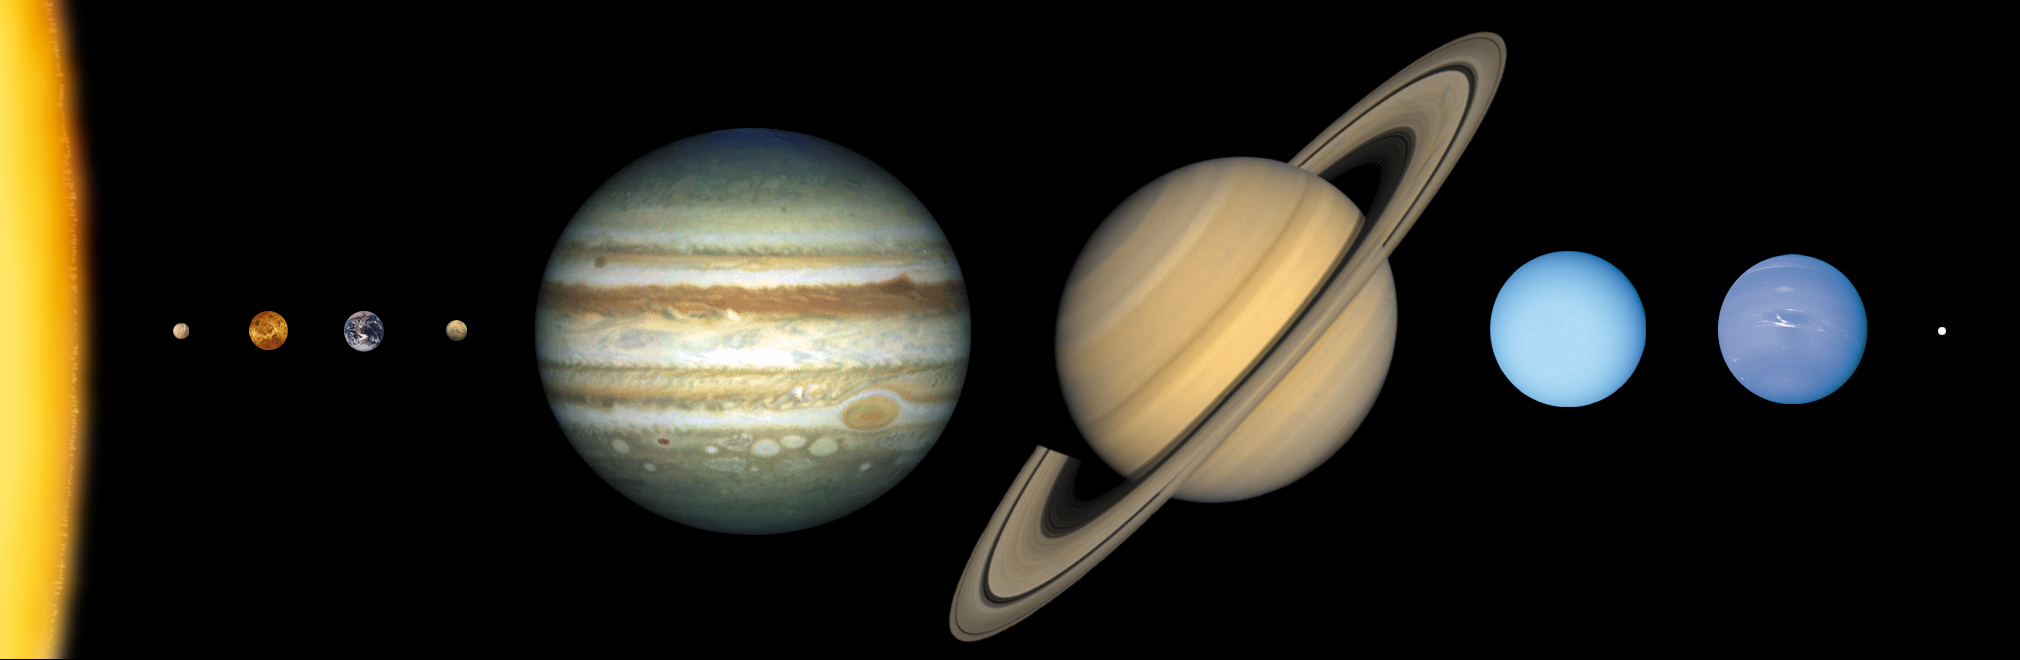
\includegraphics[width=1\linewidth]{../../pictures/Solar_system_scale.jpg}}
      \end{center}
      \captionsetup{width = 1\linewidth}
      \caption{\footnotesize Approximate sizes of the planets of our solar system relative to each other. Outward from the Sun, the planets are Mercury, Venus, Earth, Mars, Jupiter, Saturn, Uranus, Neptune, and Pluto. The planets are not shown at the appropriate distance from the Sun. Author: \href{https://commons.wikimedia.org/wiki/File:Solar_system_scale.jpg}{Lunar and Planetary Laboratory}. Public Domain.}
   %\end{adjustwidth}
\end{figure}

Such general considerations regarding certain characteristic properties appertaining to whole groups cannot, however, be applied with equal justice to the individual planets of every group, nor to the relations between the distances of the revolving planets from the central body, and their absolute size, density, period of rotation, eccentricity, and the inclination of their orbits and the axes. We know as yet of no inherent necessity, no mechanical natural law, similar to the one which teaches us that the squares of the periodic times are proportional to the cubes of the major axes, by which the above-named six elements of the planetary bodies and the form of their orbit are made dependent either on one another or on their mean distance from the Sun. Mars is smaller than the Earth and Venus, although further removed from the Sun than these last-named planets, approaching most nearly in size to Mercury, the nearest planet to the Sun. Saturn is smaller than Jupiter, and yet much larger than Uranus. The zone of the telescopic planets, which have so inconsiderable a volume, immediately precedes Jupiter (the greatest in size of any of the planetary bodies), if we consider them with regard to distance from the Sun; and yet the disks of these small asteroids, which scarcely admit of measurement, have an areal surface not much more than half that of France, Madagascar, or Borneo. However striking may be the extremely small density of all the colossal planets, which are furthest removed from the Sun, we are yet unable in this respect to recognize any regular succession.\footnote{See Kepler, on the increasing density and volume of the planets in proportion with their increase of distance from the Sun, which is described as the densest of all the heavenly bodies; in the Epitome Astron. Copern. in vii. libros digesta, 1618-1622, p. 420. Leibnitz also inclined to the opinions of Kepler and Otto von Guericke, that the planets increase in volume in proportion to their increase of distance from the Sun. See his letter to the Magdeburg Burgomaster (Mayence, 1672) in Leibnitz, Deutschen Schriften, herausg. von Guhrauer, th. i., 264.} Uranus appears to be denser than Saturn, even if we adopt the smaller mass, $\frac{1}{24005}$, assumed by Lamont; and, notwithstanding the inconsiderable difference of density observed in the innermost planetary group,\footnote{On the arrangement of masses, see Encke, in Schum., As\'{e}r. Nachr, 1843 Nr. 488, 114.} we find both Venus and Mars less dense than the Earth, which lies between them. The time of rotation certainly diminishes with increasing solar distance, but yet it is greater in Mars than in the Earth, and in Saturn than in Jupiter. The elliptic orbits of Juno, Pallas, and Mercury have the greatest degree of eccentricity, and Mars and Venus, which immediately follow each other, have the least. Mercury and Venus exhibit the same contrasts that may be observed in the four smaller planets, or asteroids, whose paths are so closely interwoven.

The eccentricities of Juno and Pallas are very nearly identical, and are each three times as great as those of Ceres and Vesta. The same may be said of the inclination of the orbits of the planets toward the plane of projection of the ecliptic, or in the position of their axes of rotation with relation to their orbits, a position on which the relations of climate, seasons of the year, and length of the days depend more than on eccentricity. Those planets that have the most elongated elliptic orbits, as Juno, Pallas, and Mercury, have also, although not to the same degree, their orbits most strongly inclined toward the ecliptic. Pallas has a comet-like inclination nearly twenty-six times greater than that of Jupiter, while in the little planet Vesta, which is so near Pallas, the angle of inclination scarcely by six times exceeds that of Jupiter. An equally irregular succession is observed in the position of the axes of the few planets (four or five) whose planes of rotation we know with any degree of certainty. It would appear from the position of the satellites of Uranus, two of which, the second and fourth, have been recently observed with certainty, that the axis of this, the outermost of all the planets, is scarcely inclined as much as 11 toward the plane of its orbit, while Saturn is placed between this planet, whose axis almost coincides with the plane of its orbit, and Jupiter, whose axis of rotation is nearly perpendicular to it.

In this enumeration of the forms which compose the world in space, we have delineated them as possessing an actual existence, and not as objects of intellectual contemplation, or as mere links of a mental and causal chain of connection. The planetary system, in its relations of absolute size and relative position of the axes, density, time of rotation, and different degrees of eccentricity of the orbits, does not appear to offer to our apprehension any stronger evidence of a natural necessity than the proportion observed in the distribution of land and water on the Earth, the configuration of continents, or the height of mountain chains. In these respects, we can discover no common law in the regions of space or in the inequalities of the earth's crust. They are facts in nature that have arisen from the conflict of manifold forces acting under unknown conditions, although man considers as accidental whatever he is unable to explain in the planetary formation on purely genetic principles. If the planets have been formed out of separate rings of vaporous matter revolving round the Sun, we may conjecture that the different thickness, unequal density, temperature, and electromagnetic tension of these rings may have given occasion to the most various agglomerations of matter, in the same manner as the amount of tangential velocity and small variations in its direction have produced so great a difference in the forms and inclinations of the elliptic orbits. Attractions of mass and laws of gravitation have no doubt exercised an influence here, no less than in the geognostic relations of the elevations of continents; but we are unable from present forms to draw any conclusions regarding the series of conditions through which they have passed. Even the so-called law of the distances of the planets from the Sun, the law of progression (which led Kepler to conjecture the existence of a planet supplying the link that was wanting in the chain of connection between Mars and Jupiter), has been found numerically inexact for the distances between Mercury, Venus, and the Earth, and at variance with the conception of a series, owing to the necessity for a supposition in the case of the first member.
The hitherto discovered principal planets that revolve round our Sun are attended certainly by fourteen, and probably by eighteen secondary planets (moons or satellites). The principal planets are, therefore, themselves the central bodies of subordinate systems. We seem to recognize in the fabric of the universe the same process of arrangement so frequently exhibited in the development of organic life, where we find in the manifold combinations of groups of plants or animals the same typical form repeated in the subordinate classes. The secondary planets or satellites are more frequent in the external region of the planetary system, lying beyond the intersecting orbits of the smaller planets or asteroids; in the inner region none of the planets are attended by satellites, with the exception of the Earth, whose moon is relatively of great magnitude, since its diameter is equal to a fourth of that of the Earth, while the diameter of the largest of all known secondary planets, the sixth satellite of Saturn, is probably about one seventeenth, and the largest of Jupiter's moons, the third, only about one twenty-sixth part that of the primary planet or central body. The planets which are attended by the largest number of satellites are most remote from the Sun and are at the same time the largest, most compressed at the poles, and the least dense. According to the most recent measurements of Madler, Uranus has a greater planetary compression than any other of the planets, viz., 544d. In our Earth and her moon, whose mean distance from one another amounts to 207,200 miles, we find that the differences of mass\footnote{If, according to Burckhardts determination, the Moon's radius be 0.2725 and its volume ,,4,,th, its density will be 05596, or nearly five ninths. Compare, also, Wilh. Beer und H. Madler, der Mond, 2,10, and Madler, Asz., 157. The material contents of the Moon are, according to Hausen, nearly 1th (and according to Madler ,.,th) that of the Earth, and its mass equal to;,4,d that of the Earth. In the largest of Jupiter's moons, the third, the relations of volume to the central body are sty ath, and of mass 5,4,,th. On the polar flattening of Uranus, see Schum., Astron. Nachr., 1844, No, 493.} and diameter between the two are much less considerable than are usually observed to exist between the principal planets and their attendant satellites, or between bodies of different orders in the solar system. While the density of the Moon is five ninths less than that of the Earth, it would appear, if we may sufficiently depend upon the determinations of their magnitudes and masses, that the second of Jupiter's moons is actually denser than that great planet itself. Among the fourteen satellites that have been investigated with any degree of certainty, the system of the seven satellites of Saturn presents an instance of the greatest possible contrast, both in absolute magnitude and in distance from the central body. The sixth of these satellites is probably not much smaller than Mars, while our moon has a diameter which does not amount to more than half that of the latter planet. With respect to volume, the two outer, the sixth and seventh of Saturn's satellites, approach the nearest to the third and brightest of Jupiter's moons. The two innermost of these satellites belong perhaps, together with the remote moons of Uranus, to the smallest cosmical bodies of our solar system, being only made visible under favorable circumstances by the most powerful instruments. They were first discovered by the forty-foot telescope of William Herschel in 1789, and were seen again by John Herschel at the Cape of Good Hope, by Vico at Rome, and by Lamont at Munich. Determinations of the true diameter of satellites, made by the measurement of the apparent size of their small disks, are subjected to many optical difficulties; but numerical astronomy, whose task it is to predetermine by calculation the motions of the heavenly bodies as they will appear when viewed from the Earth, is directed almost exelusively to motion and mass, and but little to volume.The absolute distance of a satellite from its central body isgreatest in the case of the outermost or seventh satellite ofSaturn, its distance from the body round which it revolvesamounting to more than two millions of miles, or ten times asgreat a distance as that of our moon from the Earth. In thecase of Jupiter we find that the outermost or fourth attendantmoon is only 1,040,000 miles from that planet, while the distance between Uranus and its sixth satellite (if the latter really exist) amounts to as much as 1,360,000 miles. If we compare, in each of these subordinate systems, the volume of themain planet with the distance of the orbit of its most remotesatellite, we discover the existence of entirely new numericalrelations. The distances of the outermost satellites of Uranus,Saturn, and Jupiter are, when expressed in semidiametersof the main planets, as 91, 64, and 27. The outermost satellite of Saturn appears, therefore, to be removed only aboutone fifteenth further from the center of that planet than ourmoon is from the Earth. The first or innermost of Saturnssatellites is nearer to its central body than ayy other of thesecondary planets, and presents, moreover, the only instanceof a period of revolution of less than twentyfour hours. Itsdistance from the center of Saturn may, according to Madlerand Wilhelm Beer, be expressed as 247 semidiameters of thatplanet, or as 80,088 miles. Its distance from the surface ofthe main planet is therefore 47,480 miles, and from the outermost edge of the ring only 4916 miles. The traveler mayform to himself an estimate of the smallness of this amountby remembering the statement of an enterprising navigator,Captain Beechey, that he had in three years passe over 72,800miles. If, instead of absolute distances, we take the semidiameters of the principal planets, we shall find that even thefirst or nearest of the moons of Jupiter (which is 26,000 milesfurther removed from the center of that planet than our moonis from that of the Earth) is only six semidiameters of Jupiterfrom its center, while our moon is removed from us fully 603dsemidiameters of the Earth.

In the subordinate systems of satellites, we find that the same laws of gravitation which regulate the revolutions of the principal planets round the Sun likewise govern the mutual relations existing between these planets among one another and with reference to their attendant satellites. The twelve moons of Saturn, Jupiter, and the Earth all move like the primary planets from west to east, and in elliptic orbits, deviating but little from circles. It is only in the case of one moon, and perhaps in that of the first and innermost of the satellites of Saturn (0068), that we discover an eccentricity greater than that of Jupiter; according to the very exact observations of Bessel, the eccentricity of the sixth of Saturn's satellites (0029) exceeds that of the Earth. On the extreme limits of the planetary system, where, at a distance nineteen times greater than that of our Earth, the centripetal force of the Sun is greatly diminished, the satellites of Uranus (which have certainly been but imperfectly investigated) exhibit the most striking contrasts from the facts observed with regard to other secondary planets. Instead, as in all other satellites, of having their orbits but slightly inclined toward the ecliptic and (not excepting even Saturn's ring, which may be regarded as a fusion of agglomerated satellites) moving from west to east, the satellites of Uranus are almost perpendicular to the ecliptic, and move retrogressively from east to west, as Sir John Herschel has proved by observations continued during many years. If the primary and secondary planets have been formed by the condensation of rotating rings of solar and planetary atmospheric vapor, there must have existed singular causes of retardation or impediment in the vaporous rings revolving round Uranus, by which, under relations with which we are unacquainted, the revolution of the second and fourth of its satellites was made to assume a direction opposite to that of the rotation of the central planet.